\documentclass{extbook}[14pt]
\usepackage{multicol, enumerate, enumitem, hyperref, color, soul, setspace, parskip, fancyhdr, amssymb, amsthm, amsmath, latexsym, units, mathtools}
\everymath{\displaystyle}
\usepackage[headsep=0.5cm,headheight=0cm, left=1 in,right= 1 in,top= 1 in,bottom= 1 in]{geometry}
\usepackage{dashrule}  % Package to use the command below to create lines between items
\newcommand{\litem}[1]{\item #1

\rule{\textwidth}{0.4pt}}
\pagestyle{fancy}
\lhead{}
\chead{Answer Key for Module12M Version C}
\rhead{}
\lfoot{1000-6427}
\cfoot{}
\rfoot{test}
\begin{document}
\textbf{This key should allow you to understand why you choose the option you did (beyond just getting a question right or wrong). \href{https://xronos.clas.ufl.edu/mac1105spring2020/courseDescriptionAndMisc/Exams/LearningFromResults}{More instructions on how to use this key can be found here}.}

\textbf{If you have a suggestion to make the keys better, \href{https://forms.gle/CZkbZmPbC9XALEE88}{please fill out the short survey here}.}

\textit{Note: This key is auto-generated and may contain issues and/or errors. The keys are reviewed after each exam to ensure grading is done accurately. If there are issues (like duplicate options), they are noted in the offline gradebook. The keys are a work-in-progress to give students as many resources to improve as possible.}

\rule{\textwidth}{0.4pt}

\begin{enumerate}\litem{


\textbf{General Comment:} None
}
\litem{
Using the scenario below, model the situation using an exponential function and a base of $\frac{1}{2}$. Then, solve for the half-life of the element, rounding to the nearest day.

\begin{center}
    \textit{ The half-life of an element is the amount of time it takes for the element to decay to half of its initial starting amount. There is initially 974 grams of element $X$ and after 3 years there is 108 grams remaining. }
\end{center}
The solution is \( \text{About } 0 \text{ days} \).\begin{enumerate}[label=\Alph*.]
\textbf{Plausible alternative answers include:}This uses the correct model but a base of $e$ rather than $\frac{1}{2}$.
This uses the correct model but solves for the exponential constant incorrectly.
* This is the correct option.
This models half-life as a linear function.
Please contact the coordinator if you believe all the options above are incorrect.
\end{enumerate}

\textbf{General Comment:} The model should be $A(t) = A_0 (\frac{1}{2})^{kt}$, where $A(t)$ is the amount after $t$ years, $A_0$ is the initial amount, and $k$ is decay constant. To find the half-life, you need to solve for $k$ by using the amount after $x$ years, then solve for the time $t$ when $A = \frac{A_0}{2}$. Your answer would be in years, so convert to days.
}
\litem{
For the scenario below, use the model for the volume of a cylinder as $V = \pi r^2 h$.

\begin{center}
    \textit{ Pringles wants to add 43 \text{percent} more chips to their cylinder cans and minimize the design change of their cans. They've decided that the best way to minimize the design change is to increase the radius and height by the same percentage. What should this increase be? }
\end{center}
The solution is \( \text{About } 13 \text{ percent} \).\begin{enumerate}[label=\Alph*.]
\textbf{Plausible alternative answers include:}* This is the correct option.
This corresponds to not solving for the increase properly.
This corresponds to treating both radius and height as equal contributors and not solving correctly.
This corresponds to solving correctly but treating both radius and height as equal contributors to the volume.
If you chose this, please contact the coordinator to discus how you solved the problem.
\end{enumerate}

\textbf{General Comment:} Remember that when plugging the increases of values in, you need to treat it as that percentage above 100. For example, a 5 percent increase means 105 percent.
}
\litem{
Determine the appropriate model for the graph of points below.

\begin{center}
    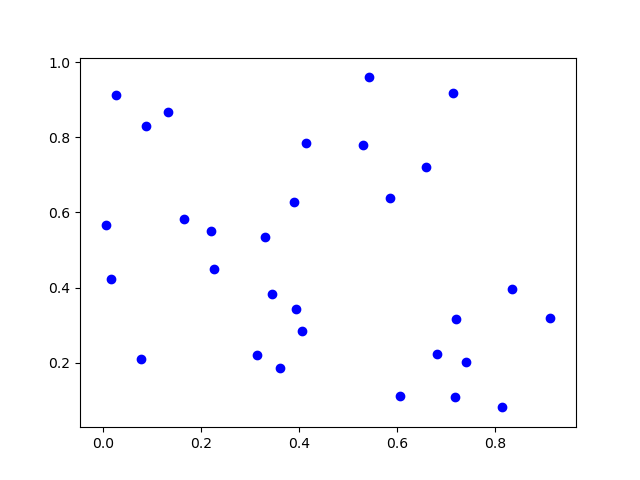
\includegraphics[width=0.5\textwidth]{../Figures/identifyModelGraph12CopyC.png}
\end{center}


The solution is \( \text{None of the above} \).\begin{enumerate}[label=\Alph*.]
\textbf{Plausible alternative answers include:}For this to be the correct option, we need to see a polynomial or rational shape.
For this to be the correct option, we want a rapid change early, then an extremely slow change later.
For this to be the correct option, we need to see a mostly straight line of points.
For this to be the correct option, we want an extremely slow change early, then a rapid change later.
For this to be the correct option, we want to see no pattern in the points.
\end{enumerate}

\textbf{General Comment:} This question is testing if you can associate the models with their graphical representation. If you are having trouble, go back to the corresponding Core module to learn about the specific function you are having trouble recognizing.
}
\litem{
For the scenario below, use the model for the volume of a cylinder as $V = \pi r^2 h$.

\begin{center}
    \textit{ Pringles wants to add 37 \text{percent} more chips to their cylinder cans and minimize the design change of their cans. They've decided that the best way to minimize the design change is to increase the radius and height by the same percentage. What should this increase be? }
\end{center}
The solution is \( \text{About } 11 \text{ percent} \).\begin{enumerate}[label=\Alph*.]
\textbf{Plausible alternative answers include:}This corresponds to solving correctly but treating both radius and height as equal contributors to the volume.
This corresponds to not solving for the increase properly.
This corresponds to treating both radius and height as equal contributors and not solving correctly.
* This is the correct option.
If you chose this, please contact the coordinator to discus how you solved the problem.
\end{enumerate}

\textbf{General Comment:} Remember that when plugging the increases of values in, you need to treat it as that percentage above 100. For example, a 5 percent increase means 105 percent.
}
\litem{
Determine the appropriate model for the graph of points below.

\begin{center}
    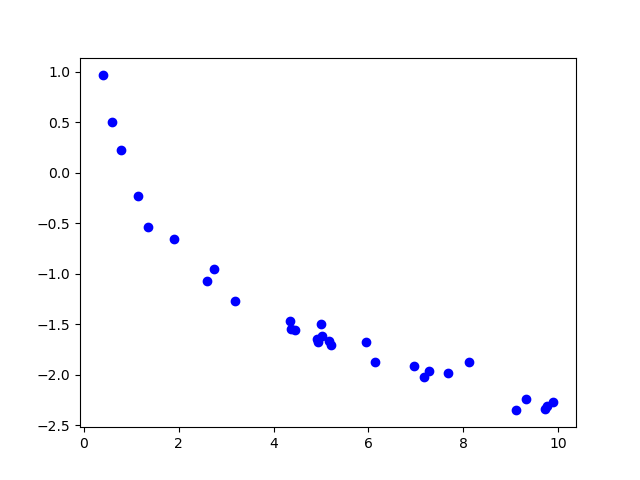
\includegraphics[width=0.5\textwidth]{../Figures/identifyModelGraph12C.png}
\end{center}


The solution is \( \text{Exponential model} \).\begin{enumerate}[label=\Alph*.]
\textbf{Plausible alternative answers include:}For this to be the correct option, we want a rapid change early, then an extremely slow change later.
For this to be the correct option, we want an extremely slow change early, then a rapid change later.
For this to be the correct option, we need to see a polynomial or rational shape.
For this to be the correct option, we need to see a mostly straight line of points.
For this to be the correct option, we want to see no pattern in the points.
\end{enumerate}

\textbf{General Comment:} This question is testing if you can associate the models with their graphical representation. If you are having trouble, go back to the corresponding Core module to learn about the specific function you are having trouble recognizing.
}
\litem{
Solve the modeling problem below, if possible.

\begin{center}
    \textit{ In CHM2045L, Brittany created a 18 liter 25 percent solution of chemical $\chi$ using two different solution percentages of chemical $\chi$. When she went to write her lab report, she realized she forgot to write the amount of each solution she used! If she remembers she used 15 percent and 43 percent solutions, what was the amount she used of the 43 percent solution? }
\end{center}
The solution is \( 6.43 liters \).\begin{enumerate}[label=\Alph*.]
\textbf{Plausible alternative answers include:}This would be correct if Brittany used equal parts of each solution.
This is the concentration of 15 percent solution.
This was a random value. If this was not a guess, contact the coordinator to talk about how you got this value.
*This is the correct option.
You may have chose this if you thought you needed to know how much of the second solution was used in the problem. Remember that the total minus the first solution would give you the second amount used.
\end{enumerate}

\textbf{General Comment:} Build the model exactly as you did in Module 9M. Then, solve for the volume you are looking for.
}
\litem{
Solve the modeling problem below, if possible.

\begin{center}
    \textit{ A new virus is spreading throughout the world. There were initially 8 many cases reported, but the number of confirmed cases has quadrupled every 5 days. How long will it be until there are at least 10000 confirmed cases? }
\end{center}
The solution is \( \text{About } 26 \text{ days} \).\begin{enumerate}[label=\Alph*.]
\textbf{Plausible alternative answers include:}You modeled the situation with $e$ as the base and did not apply the properties of log correctly.
* This is the correct option.
You modeled the situation with $e$ as the base, but solved correctly otherwise.
You modeled the situation correctly but did not apply the properties of log correctly.
If you chose this option, please contact the coordinator to discuss why you think this is the case.
\end{enumerate}

\textbf{General Comment:} Set up the model the same as in Module 11M. Then, plug in 10000 and solve for $d$ in your model.
}
\litem{
Solve the modeling problem below, if possible.

\begin{center}
    \textit{ In CHM2045L, Brittany created a 19 liter 19 percent solution of chemical $\chi$ using two different solution percentages of chemical $\chi$. When she went to write her lab report, she realized she forgot to write the amount of each solution she used! If she remembers she used 18 percent and 33 percent solutions, what was the amount she used of the 33 percent solution? }
\end{center}
The solution is \( 1.27 liters \).\begin{enumerate}[label=\Alph*.]
\textbf{Plausible alternative answers include:}*This is the correct option.
This is the concentration of 18 percent solution.
This would be correct if Brittany used equal parts of each solution.
This was a random value. If this was not a guess, contact the coordinator to talk about how you got this value.
You may have chose this if you thought you needed to know how much of the second solution was used in the problem. Remember that the total minus the first solution would give you the second amount used.
\end{enumerate}

\textbf{General Comment:} Build the model exactly as you did in Module 9M. Then, solve for the volume you are looking for.
}
\litem{
Solve the modeling problem below, if possible.

\begin{center}
    \textit{ A new virus is spreading throughout the world. There were initially 5 many cases reported, but the number of confirmed cases has tripled every 2 days. How long will it be until there are at least 10000 confirmed cases? }
\end{center}
The solution is \( \text{About } 14 \text{ days} \).\begin{enumerate}[label=\Alph*.]
\textbf{Plausible alternative answers include:}You modeled the situation with $e$ as the base, but solved correctly otherwise.
You modeled the situation with $e$ as the base and did not apply the properties of log correctly.
You modeled the situation correctly but did not apply the properties of log correctly.
* This is the correct option.
If you chose this option, please contact the coordinator to discuss why you think this is the case.
\end{enumerate}

\textbf{General Comment:} Set up the model the same as in Module 11M. Then, plug in 10000 and solve for $d$ in your model.
}
\end{enumerate}

\end{document}